\documentclass[tikz,border=8pt]{standalone}
% Shared look for every TikZ diagram. Load with \input{../../tools/tikz-style.tex}
\usepackage[sfdefault]{roboto}
\usetikzlibrary{arrows.meta, positioning, shapes.geometric, calc, fit, backgrounds}
\definecolor{cblue}{HTML}{4C78A8}
\definecolor{corange}{HTML}{F58518}
\definecolor{cgreen}{HTML}{54A24B}
\definecolor{cred}{HTML}{E45756}
\definecolor{cpurple}{HTML}{B279A2}
\definecolor{cgrey}{HTML}{6B6B6B}
\tikzset{
  every picture/.style={font=\sffamily, line width=1.2pt},
  box/.style={draw=#1, fill=#1!12, rounded corners=4pt, align=center, inner sep=7pt, minimum height=1.1cm},
  box/.default=cgrey,
  arrow/.style={-{Stealth[length=3mm]}, draw=cgrey, line width=1.4pt},
  title/.style={font=\sffamily\bfseries\Large},
  note/.style={font=\sffamily\small, text=cgrey, align=center},
}
\AtBeginDocument{\hyphenpenalty=10000 \exhyphenpenalty=10000}

% The four engines, each with its default step, contact model and solver, from its documentation (read 2026-10-12):
% MuJoCo (XML reference: timestep 0.002, integrator Euler = semi-implicit, cone pyramidal, solver Newton; soft
% contact, solref 0.02 1); Gazebo Sim (physics page: DART by default, collision detector ode, solver dantzig;
% SDFormat 1.11: max_step_size 0.001, real_time_factor 1, friction mu 1); Isaac Sim (simulation fundamentals: PhysX,
% 60 steps per second by default; solvers PGS and TGS); Drake (MultibodyPlantConfig: time_step 0.001,
% contact_model hydroelastic_with_fallback, discrete approximation lagged, penetration_allowance 0.001 m).
\begin{document}
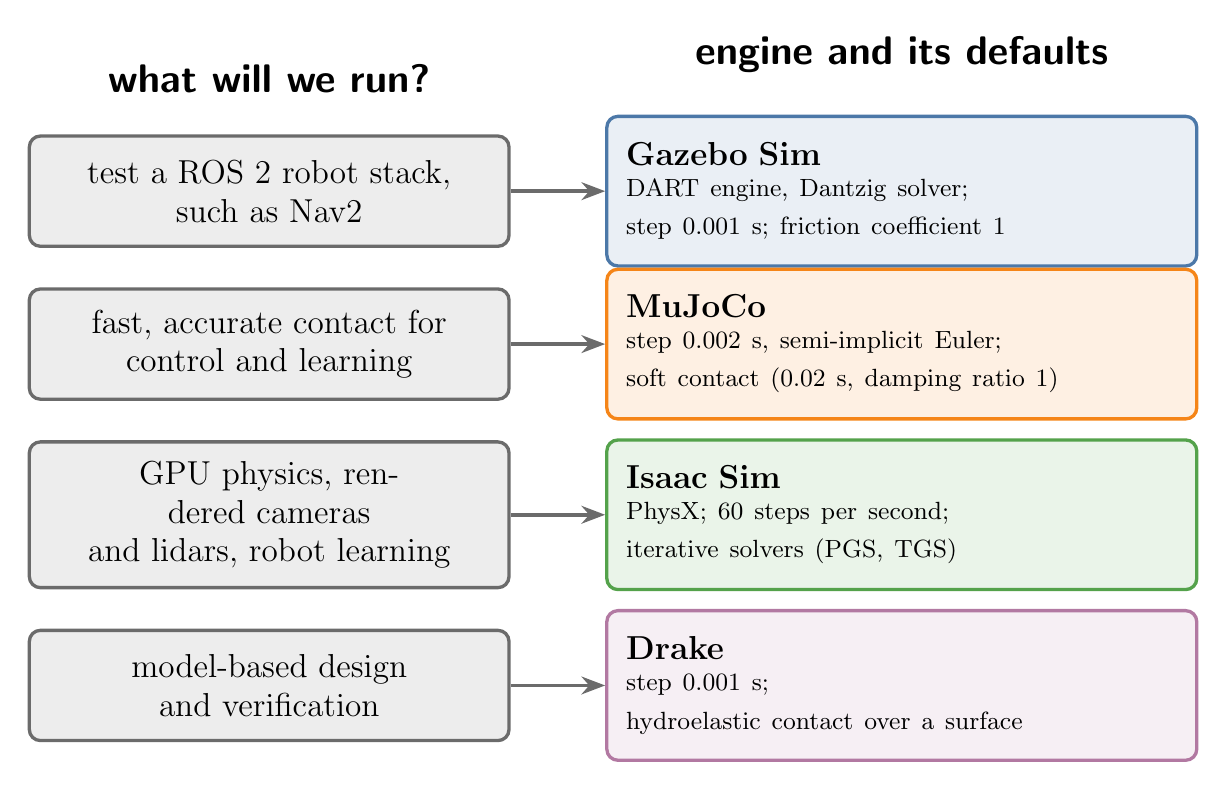
\begin{tikzpicture}[every node/.append style={font=\large}, node distance=0.5cm,
  q/.style={box=cgrey, minimum width=6.0cm, text width=5.6cm, minimum height=1.4cm},
  e/.style={box=#1, minimum width=7.4cm, text width=7.0cm, minimum height=1.9cm, align=left}]
  \node[q] (q1) {test a ROS 2 robot stack,\\ such as Nav2};
  \node[q, below=of q1] (q2) {fast, accurate contact for\\ control and learning};
  \node[q, below=of q2] (q3) {GPU physics, rendered cameras\\ and lidars, robot learning};
  \node[q, below=of q3] (q4) {model-based design\\ and verification};
  \node[e=cblue, right=1.2cm of q1] (e1) {\textbf{Gazebo Sim}\\ \small DART engine, Dantzig solver;\\ \small step 0.001 s; friction coefficient 1};
  \node[e=corange, right=1.2cm of q2] (e2) {\textbf{MuJoCo}\\ \small step 0.002 s, semi-implicit Euler;\\ \small soft contact (0.02 s, damping ratio 1)};
  \node[e=cgreen, right=1.2cm of q3] (e3) {\textbf{Isaac Sim}\\ \small PhysX; 60 steps per second;\\ \small iterative solvers (PGS, TGS)};
  \node[e=cpurple, right=1.2cm of q4] (e4) {\textbf{Drake}\\ \small step 0.001 s;\\ \small hydroelastic contact over a surface};
  \foreach \i in {1,2,3,4} {\draw[arrow] (q\i) -- (e\i);}
  \node[title, above=0.4cm of q1] {what will we run?};
  \node[title, above=0.4cm of e1] {engine and its defaults};
\end{tikzpicture}
\end{document}
